\markboth{}{}

\begin{figure}[H]
    \center
    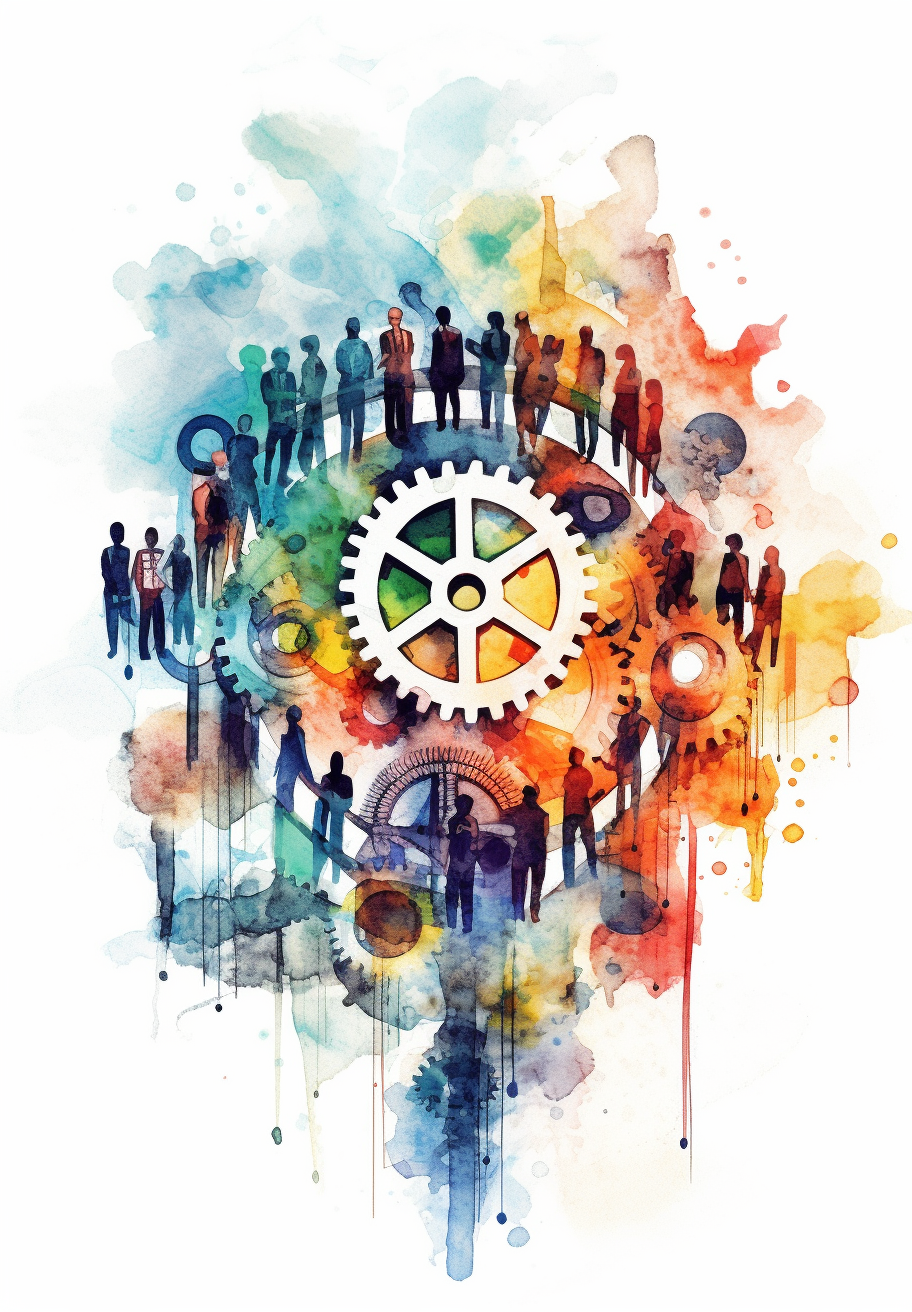
\includegraphics[keepaspectratio, width=\textwidth, height=\textheight]{images/07be4a47-3beb-4a74-a68f-7c7382e8930f.png}
    \caption{Aquarelle représentant différentes manières d'organiser différentes équipes.\\
        Image générée par Kevin Delfour sur Midjourney.}
\end{figure}
\newpage

\chapter{Les alternatives au modèle d'entreprise libérée}

Alors que le modèle d'entreprise libérée a certainement sa place dans le panorama contemporain du management, il serait réducteur de l'ériger comme la seule voie vers un environnement de travail plus égalitaire, autonome et épanouissant. En effet, une pléthore d'autres formes d'organisation et de management existent, chacune offrant ses propres avantages et inconvénients, ainsi que ses propres réponses à la question de l'autonomie, de la participation et du bien-être des employés. Cela illustre bien l'idée que le management est un domaine dynamique, innovant et diversifié, où de nouvelles idées et approches sont constamment explorées et mises en pratique\footnote{Cunliffe, A. L. (2009). The philosopher leader: On relationalism, ethics and reflexivity—a critical perspective to teaching leadership. Management Learning, 40(1), 87-101.}.

\section{Les autres formes d'organisation et de management}

De nombreuses autres formes d'organisation et de management cherchent à redéfinir la relation entre les employés et leurs lieux de travail, en se concentrant sur l'autonomie, la participation, le bien-être et la performance. Elles offrent des alternatives intéressantes au modèle d'entreprise libérée.

\subsection{L'autogestion}

L'autogestion est une forme d'organisation où les employés contrôlent directement et collectivement leur lieu de travail\footnote{Rothschild, J., \& Whitt, J. A. (1986). The cooperative workplace. Cambridge University Press.}. Ce type de structure est souvent utilisé dans les coopératives de travailleurs, où les employés sont également propriétaires de l'entreprise. Il n'y a pas de gestionnaires au sens traditionnel du terme ; les décisions sont prises démocratiquement, souvent par le biais de réunions de travailleurs.

\subsection{L'entreprise démocratique}

Dans une entreprise démocratique, les employés participent activement aux décisions de l'entreprise. Ce modèle s'inspire des principes démocratiques pour créer une culture d'égalité et de participation\footnote{Semler, R. (2003). The Seven-Day Weekend: Changing the Way Work Works. Portfolio.}. Les employés peuvent voter sur diverses questions, comme la stratégie de l'entreprise, l'allocation des ressources et même la sélection des dirigeants.

\subsection{L'entreprise sociocratique}

La sociocratie est un système de gouvernance basé sur le consentement et l'égalité du pouvoir\footnote{Endenburg, G. (1998). Sociocracy: The organization of decision-making, "no objection!" as the principle of sociocracy. Eburon.}. Elle repose sur des cercles de décision semi-autonomes, où chaque membre a une voix égale dans le processus de prise de décision. Ce modèle vise à faciliter la coopération, l'innovation et le respect au sein de l'entreprise.

Chacune de ces alternatives offre sa propre approche pour créer un environnement de travail plus égalitaire et autonome. Cependant, comme le modèle d'entreprise libérée, elles ne sont pas sans défis et exigent une attention particulière à la mise en œuvre et à la gestion.

\section{Les innovations et les expérimentations en cours}

Dans le monde des affaires dynamique et en constante évolution d'aujourd'hui, de nombreuses entreprises cherchent à repousser les limites de ce qui est possible en matière d'organisation et de management. Ces expérimentations, souvent guidées par des principes d'agilité, de responsabilité et d'autonomie, peuvent offrir des aperçus intéressants de l'avenir du travail.

L'une de ces innovations est le concept d'entreprise teal, popularisé par Frédéric Laloux dans son livre "Reinventing Organizations"\footnote{Laloux, F. (2014). Reinventing Organizations. Nelson Parker.}. Les organisations teal se caractérisent par leur autogestion, leur orientation vers la réalisation du potentiel humain et leur vision évolutive du monde.

Une autre tendance notable est l'adoption de modèles d'organisation agiles, en particulier dans le secteur de la technologie. Ces modèles sont axés sur la réactivité, la flexibilité et la collaboration, avec des équipes autogérées qui travaillent sur des projets en cycles courts et itératifs.

Enfin, certains suggèrent que le futur du travail pourrait être caractérisé par des organisations plus distribuées et décentralisées, avec des équipes de travail dispersées géographiquement et une plus grande utilisation des technologies numériques pour la collaboration\footnote{Hinds, P. J., \& Kiesler, S. (Eds.). (2002). Distributed work. MIT Press.}.

Chacune de ces expérimentations offre une perspective unique sur la manière dont les organisations pourraient évoluer à l'avenir. Cependant, il est important de noter que ces innovations sont encore en cours d'exploration et de développement, et que leurs implications à long terme restent incertaines.

\section{Les perspectives d'évolution du modèle d'entreprise libérée}

Le modèle d'entreprise libérée, malgré les critiques et les défis qu'il a rencontrés, est loin d'être figé. De nombreuses entreprises qui ont adopté ce modèle continuent de l'adapter et de l'évoluer en fonction de leurs besoins spécifiques, de leurs expériences et des retours de leurs employés.

Il est probable que nous verrons de nombreuses variations sur le thème de l'entreprise libérée dans les années à venir. Certaines entreprises pourraient chercher à fusionner le modèle d'entreprise libérée avec d'autres approches de management, créant ainsi des hybrides uniques qui combinent le meilleur de plusieurs mondes. Par exemple, l'idée d'une entreprise libérée pourrait être combinée avec les principes de l'agilité, créant une organisation qui est non seulement autonome, mais aussi hautement réactive et adaptable\footnote{Denning, S. (2018). Age of Agile. Amacom.}.

D'autres pourraient chercher à appliquer les principes de l'entreprise libérée à différents niveaux de l'organisation, créant ainsi des "îlots de liberté" au sein de structures plus traditionnelles. Cela pourrait permettre une plus grande expérimentation et adaptation, tout en minimisant les risques associés à une transformation complète de l'entreprise\footnote{Getz, I. (2011). Freedom, Inc.: Free Your Employees and Let Them Lead Your Business for Greater Success. Crown Business.}.

Dans tous les cas, il est clair que le modèle d'entreprise libérée a stimulé une réflexion importante sur la manière dont les entreprises sont gérées et organisées. Il continuera probablement à influencer le discours et la pratique du management dans un avenir proche, même si sa forme et son application peuvent évoluer.
